% LaTeX source for ``Python for Informatics: Exploring Information''
% Copyright (c)  2010-  Charles R. Severance, All Rights Reserved

\chapter{Ejecución condicional}

\section{Expresiones booleanas}
\index{booleana, expresión}
\index{expresión!booleana}
\index{lógico, operador}
\index{operador!lógico}

Una {\bf expresión booleana} es aquella que puede ser verdadera ({\tt True})
o falsa ({\tt False}). Los ejemplos siguientes usan el operador
{\tt ==}, que compara dos operandos y devuelve
{\tt True} si son iguales y {\tt False} en caso contrario:

\beforeverb
\begin{verbatim}
>>> 5 == 5
True
>>> 5 == 6
False
\end{verbatim}
\afterverb
%
{\tt True} y {\tt False} son valores especiales
que pertenecen al tipo {\tt bool (booleano)}; no son cadenas:

\index{True, valor especial}
\index{False, valor especial}
\index{valor especial!True}
\index{valor especial!False}
\index{booleano, tipo}
\index{tipo!booleano}

\beforeverb
\begin{verbatim}
>>> type(True)
<type 'bool'>
>>> type(False)
<type 'bool'>
\end{verbatim}
\afterverb
%
El operador {\tt ==} es uno de los {\bf operadores de comparación};
los demás son:

\beforeverb
\begin{verbatim}
      x != y               # x es distinto de y
      x > y                # x es mayor que y
      x < y                # x es menor que y
      x >= y               # x es mayor o igual que y
      x <= y               # x es menor o igual que y
      x is y               # x es lo mismo que y
      x is not y           # x no es lo mismo que y
\end{verbatim}
\afterverb
%
A pesar de que estas operaciones probablemente te resulten familiares, los
símbolos en Python son diferentes de los símbolos matemáticos que se usan
para realizar las mismas operaciones. Un error muy común
es usar sólo un símbolo igual ({\tt =}) en vez del símbolo de doble igualdad
({\tt ==}). Recuerda que {\tt =} es un operador de asignación, y
{\tt ==} es un operador de comparación. No existe algo como
{\tt \verb"=<"} o {\tt \verb"=>"}.

\index{comparación!operador}
\index{operador!comparación}


\section {Operadores lógicos}
\index{lógico, operador}
\index{operador!lógico}

Existen tres {\bf operadores lógicos}: {\tt and (y)}, {\tt
or (o)}, y {\tt not (no)}. El significado semántico de estas operaciones
es similar a su significado en inglés. Por ejemplo, 

{\tt x > 0 and x < 10} 

es verdadero sólo cuando {\tt x} es mayor que 0
\emph{y} menor que 10.

\index{and, operador}
\index{or, operador}
\index{not, operador}
\index{operador!and}
\index{operador!or}
\index{operador!not}

{\tt n\%2 == 0 or n\%3 == 0} es verdadero si \emph{cualquiera} de las condiciones
es verdadera, es decir, si el número es divisible por 2 \emph{o} por 3.

Finalmente, el operador {\tt not} niega una expresión
booleana, de modo que {\tt not (x > y)} es verdadero si {\tt x > y} es falso;
es decir, si {\tt x} es menor o igual que {\tt y}.

Estrictamente hablando, los operandos de los operadores lógicos deberían ser
expresiones booleanas, pero Python no es muy estricto.
Cualquier número distinto de cero se interpreta como ``verdadero.''

\beforeverb
\begin{verbatim}
>>> 17 and True
True
\end{verbatim}
\afterverb
%
Esta flexibilidad puede ser útil, pero existen ciertas sutilezas en ese tipo de uso
que pueden resultar confusas. Es posible que prefieras evitar usarlo de este modo
hasta que estés bien seguro de lo que estás haciendo.

\section{Ejecución condicional}
\label{conditional execution}

\index{condicional!sentencia}
\index{sentencia!condicional}
\index{if, sentencia}
\index{sentencia!if}
\index{condicional!ejecución}

Para poder escribir programas útiles, casi siempre vamos a necesitar
la capacidad de comprobar condiciones y cambiar el comportamiento del programa
de acuerdo a ellas. Las {\tt sentencias condicionales} nos proporciona esa capacidad.
La forma más sencilla es la sentencia {\tt if}:

\beforeverb
\begin{verbatim}
if x > 0 :
    print 'x es positivo'
\end{verbatim}
\afterverb
%
La expresión booleana después de la sentencia {\tt if} recibe
el nombre de {\bf condición}. La sentencia {\tt if} se finaliza
con un carácter de dos-puntos (:) y la(s) línea(s) que van detrás de
la sentencia if van indentadas\footnote{el término correcto en español
sería ``sangradas'', pero en el mundillo de la programación se suele
decir que las líneas van ``indentadas'' (Nota del trad.)}
(es decir, llevan una tabulación o varios espacios en blanco al principio).

\beforefig
\centerline{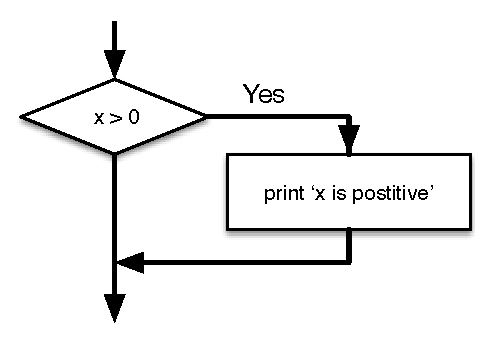
\includegraphics[height=1.75in]{figs2/if.eps}}
\afterfig

Si la condición lógica es verdadera, la sentencia indentada
será ejecutada. Si la condición es falsa,
la sentencia indentada será omitida.

\index{condición}
\index{compuesta, sentencia}
\index{sentencia!compuesta}

La sentencia {\tt if} tiene la misma estructura que la definición de funciones
o los bucles {\tt for}\footnote{Estudiaremos las funciones en el capítulo 4
y los bucles en el capítulo 5.}. La sentencia consiste en una línea de encabezado
que termina con el carácter dos-puntos (:)
seguido por un bloque indentado. Las sentencias de este tipo
reciben el nombre de {\bf sentencias compuestas}, porque se extienden
a lo largo de varias líneas.

No hay límite en el número de sentencias que pueden aparecer en el
cuerpo, pero debe haber al menos una.
Ocasionalmente, puede resultar útil tener un cuerpo sin sentencias
(normalmente como emplazamiento reservado para código que no se ha escrito aún). En ese
caso, se puede usar la sentencia {\tt pass}, que no hace nada.

\index{pass, sentencia}
\index{sentencia!pass}

\beforeverb
\begin{verbatim}
if x < 0 :
    pass          # ¡necesito gestionar los valores negativos!
\end{verbatim}
\afterverb
%
Si introduces una sentencia {\tt if} en el intérprete de Python, el prompt cambiará
su aspecto habitual por puntos suspensivos, para indicar que estás en medio de un bloque de sentencias, como
se muestra a continuación:

\beforeverb
\begin{verbatim}
>>> x = 3
>>> if x < 10:
...    print 'Pequeño'
... 
Pequeño
>>>
\end{verbatim}
\afterverb
%

\section{Ejecución alternativa}
\label{alternative execution}

\index{ejecución alternativa}
\index{else, palabra clave}
\index{palabra clave!else}

La segunda forma de la sentencia {\tt if} es la {\bf ejecución alternativa},
en la cual existen dos posibilidades y la condición determina
cual de ellas será ejecutada. La sintaxis es similar a ésta:

\beforeverb
\begin{verbatim}
if x%2 == 0 :
    print 'x es par'
else :
    print 'x es impar'
\end{verbatim}
\afterverb
%
Si al dividir {\tt x} por 2 obtenemos como resto 0, entonces sabemos
que {\tt x} es par, y el programa muestra un mensaje a tal
efecto. Si esa condición es falsa, se ejecuta el segundo
conjunto de sentencias.

\beforefig
\centerline{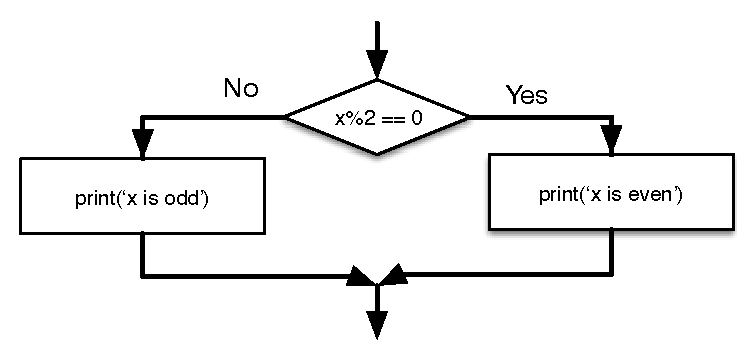
\includegraphics[height=1.75in]{figs2/if-else.eps}}
\afterfig

Dado que la condición debe ser obligatoriamente verdadera o falsa, solamente una de
las alternativas será ejecutada. Las alternativas reciben el nombre de
{\bf ramas}, dado que se trata de ramificaciones en el flujo de la ejecución.

\index{rama}

\section{Condicionales encadenados}
\index{encadenado, condicional}
\index{condicional!encadenado}

Algunas veces hay más de dos posibilidades, de modo que necesitamos más
de dos ramas. Una forma de expresar una operación como ésa es usar un
{\bf condicional encadenado}:

\beforeverb
\begin{verbatim}
if x < y:
    print 'x es menor que y'
elif x > y:
    print 'x es mayor que y'
else:
    print 'x e y son iguales'
\end{verbatim}
\afterverb
%
{\tt elif} es una abreviatura para ``else if''.  En este caso también
será ejecutada únicamente una de las ramas.

\beforefig
\centerline{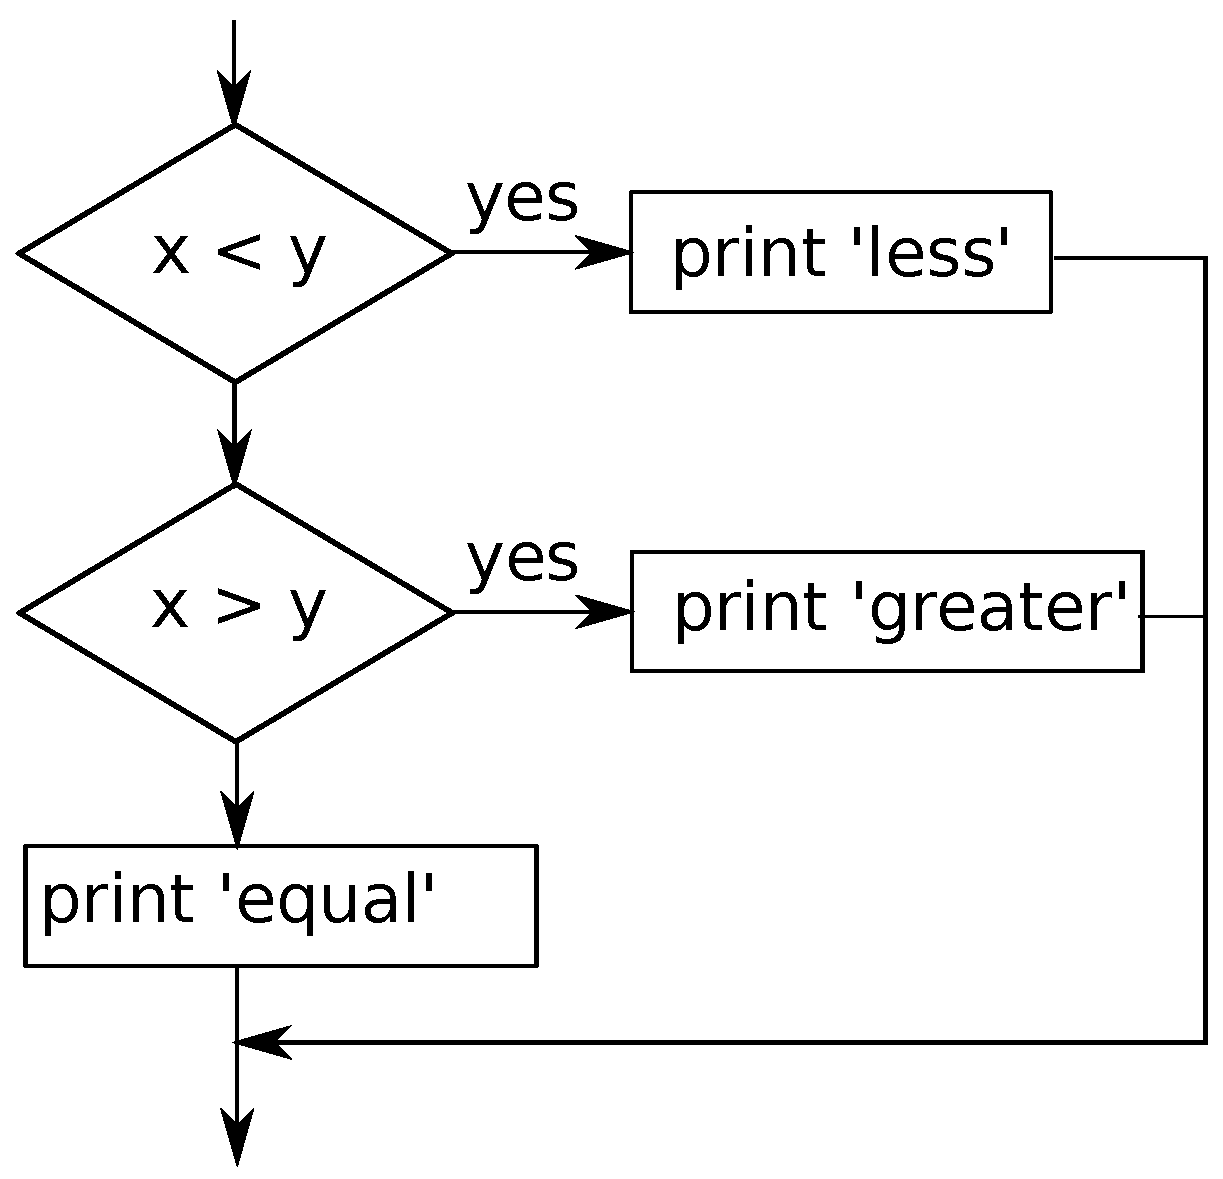
\includegraphics[height=3.00in]{figs2/elif.eps}}
\afterfig

No hay un límite para el número de sentencias
{\tt elif}. Si hay una clausula {\tt else}, debe ir
al final, pero tampoco es obligatorio que ésta exista.

\index{elif, palabra clave}
\index{palabra clave!elif}


\beforeverb
\begin{verbatim}
if choice == 'a':
    print 'Respuesta incorrecta'
elif choice == 'b':
    print 'Respuesta correcta'
elif choice == 'c':
    print 'Casi, pero no es correcto'
\end{verbatim}
\afterverb
%
Cada condición es comprobada en orden. Si la primera es falsa,
se comprueba la siguiente y así con las demás. Si una de ellas es
verdadera, se ejecuta la rama correspondiente, y la sentencia
termina. Incluso si hay más de una condición que sea verdadera, sólo se
ejecuta la primera que se encuentra.

\section{Condicionales anidados}
\index{anidado, condicional}
\index{condicional!anidado}

Un condicional puede también estar anidado dentro de otro. Podríamos
haber escrito el ejemplo anterior de las tres ramas de este modo:

\beforeverb
\begin{verbatim}
if x == y:
    print 'x e y son iguales'
else:
    if x < y:
        print 'x es menor que y'
    else:
        print 'x es mayor que y'
\end{verbatim}
\afterverb
%
El condicional exterior contiene dos ramas. La
primera rama ejecuta una sentencia simple. La segunda
contiene otra sentencia {\tt if}, que tiene a su vez sus propias
dos ramas. Esas dos ramas son ambas sentencias simples,
pero podrían haber sido sentencias condicionales también.

\beforefig
\centerline{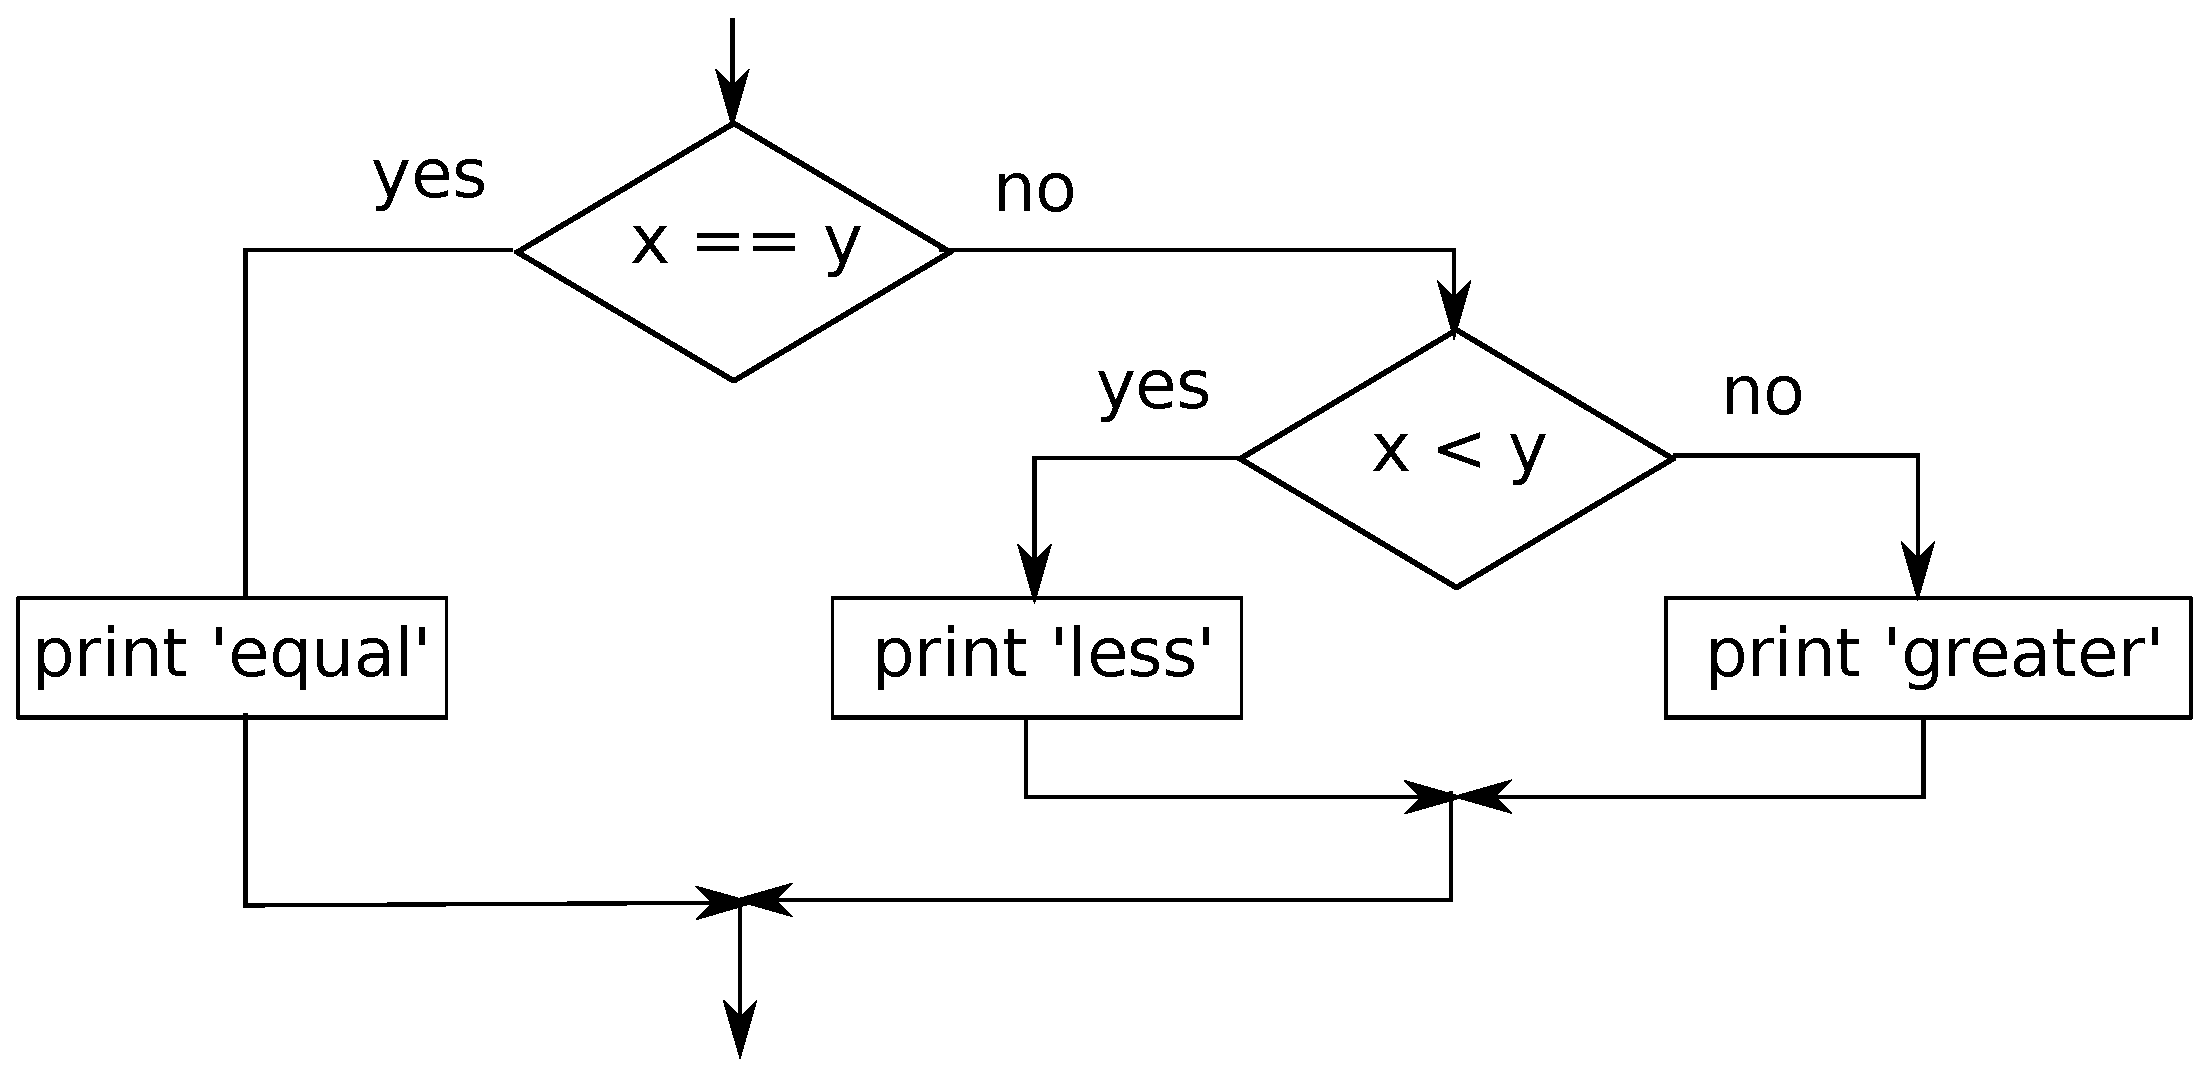
\includegraphics[height=2.50in]{figs2/nested.eps}}
\afterfig

A pesar de que el indentado de las sentencias hace que la estructura
esté clara, los {\bf condicionales anidados} pueden volverse difíciles
de leer rápidamente. En general, es buena idea evitarlos si se puede.

Los operadores lógicos a menudo proporcionan un modo de simplificar las
sentencias condicionales anidadas. Por ejemplo, el código siguiente
puede ser reescrito usando un único condicional:

\beforeverb
\begin{verbatim}
if 0 < x:
    if x < 10:
        print 'x es un número positivo con un sólo dígito.'
\end{verbatim}
\afterverb
%
La sentencia {\tt print} se ejecuta solamente si se cumplen las dos condiciones
anteriores, así que en realidad podemos conseguir el mismo efecto con el operador {\tt and}:

\beforeverb
\begin{verbatim}
if 0 < x and x < 10:
    print 'x es un número positivo con un sólo dígito.'
\end{verbatim}
\afterverb


\section{Captura de excepciones usando try y except}
\label{catch1}

Anteriormente vimos un fragmento de código donde usábamos las funciones \verb"raw_input" e
{\tt int} para leer y analizar un número entero introducido por
el usuario. También vimos lo poco seguro que podía llegar a resultar hacer algo así:

\beforeverb
\begin{verbatim}
>>> velocidad = raw_input(prompt)
¿Cual.... es la velocidad de vuelo de una golondrina sin carga?
¿Te refieres a una golondrina africana o a una europea?
>>> int(velocidad)
ValueError: invalid literal for int()
>>>
\end{verbatim}
\afterverb
%
Cuando estamos trabajando con el intérprete de Python, tras el error simplemente
nos aparece de nuevo el prompt, así que pensamos ``¡epa, me he equivocado!'', y continuamos
con la siguiente sentencia.

Sin embargo, si se escribe ese código en un
script de Python y se produce el error, el script se detendrá
inmediatamente, y mostrará un ``traceback''.
No ejecutará la siguiente sentencia.

\index{traceback}

He aquí un programa de ejemplo para convertir una temperatura
desde grados Fahrenheit a grados Celsius:

\index{fahrenheit}
\index{celsius}
\index{conversión de temperatura}

\beforeverb
\begin{verbatim}
ent = raw_input('Introduzca la Temperatura Fahrenheit:')
fahr = float(ent)
cel = (fahr - 32.0) * 5.0 / 9.0
print cel
\end{verbatim}
\afterverb
%
Si ejecutamos este código y le damos una entrada no válida, simplemente
fallará con un mensaje de error bastante antipático:

\beforeverb
\begin{verbatim}
python fahren.py 
Introduzca la Temperatura Fahrenheit:72
22.2222222222

python fahren.py 
Introduzca la Temperatura Fahrenheit:fred
Traceback (most recent call last):
  File "fahren.py", line 2, in <module>
    fahr = float(ent)
ValueError: invalid literal for float(): fred
\end{verbatim}
\afterverb
%
Existen estructuras de ejecución condicional dentro de
Python para manejar este tipo de errores esperados e
inesperados, llamadas ``try / except''. La idea de {\tt try}
y {\tt except} es que si se sabe que cierta secuencia
de instrucciones puede generar un problema, sea posible
añadir ciertas sentencias para que sean ejecutadas en caso de error.
Estas sentencias extras (el bloque except) serán ignoradas
si no se produce ningún error.

Puedes pensar en la característica {\tt try} y {\tt except}
de Python como una ``póliza de seguros'' en una secuencia
de sentencias.

Se puede reescribir nuestro conversor de temperaturas de esta forma:

\beforeverb
\begin{verbatim}
ent = raw_input('Introduzca la Temperatura Fahrenheit:')
try:
    fahr = float(ent)
    cel = (fahr - 32.0) * 5.0 / 9.0
    print cel
except:
    print 'Por favor, introduzca un número'
\end{verbatim}
\afterverb
%

Python comienza ejecutando la
secuencia de sentencias del bloque
{\tt try}. Si todo va bien, se
saltará todo el bloque {\tt except} y terminará.
Si ocurre una excepción dentro del bloque {\tt try},
Python saltará fuera de ese bloque y
ejecutará la secuencia de sentencias del bloque {\tt except}.

\beforeverb
\begin{verbatim}
python fahren2.py 
Introduzca la Temperatura Fahrenheit:72
22.2222222222

python fahren2.py 
Introduzca la Temperatura Fahrenheit:fred
Por favor, introduzca un número
\end{verbatim}
\afterverb
%

Gestionar una excepción con una sentencia {\tt try} recibe el nombre de
{\bf capturar} una excepción. En este ejemplo, la clausula {\tt except}
muestra un mensaje de error. En general,
capturar una excepción te da la oportunidad de corregir el problema,
volverlo a intentar o, al menos, terminar el programa con elegancia.

\section{Evaluación en cortocircuito de expresiones lógicas}
\index{cortocircuito}

Cuando Python está procesando una expresión lógica, como
{\tt x >= 2 and (x/y) > 2}, evalúa la expresión de
izquierda a derecha. Debido a la definición de {\tt and},
si {\tt x} es menor de 2, la expresión {\tt x >= 2} resulta ser
{\tt falsa}, de modo que la expresión completa ya va a resultar {\tt falsa}, independientemente
de si {\tt (x/y) > 2} se evalúa como {\tt verdadera} o {\tt falsa}.

Cuando Python detecta que no se gana nada evaluando
el resto de una expresión lógica, detiene su evaluación y no
realiza el cálculo del resto de la expresión.
Cuando la evaluación de una expresión lógica se detiene debido a que
ya se conoce el valor final, eso es conocido como {\bf cortocircuitar}
la evaluación.

\index{guardián, patrón}
\index{patrón!guardián}
A pesar de que esto pueda parecer hilar demasiado fino, el funcionamiento
en cortocircuito nos descubre una ingeniosa técnica conocida como {\bf patrón guardián}.
Examina la siguiente secuencia de código en el intérprete de Python:

\beforeverb
\begin{verbatim}
>>> x = 6 
>>> y = 2
>>> x >= 2 and (x/y) > 2
True
>>> x = 1 
>>> y = 0
>>> x >= 2 and (x/y) > 2
False
>>> x = 6
>>> y = 0
>>> x >= 2 and (x/y) > 2
Traceback (most recent call last):
  File "<stdin>", line 1, in <module>
ZeroDivisionError: integer division or modulo by zero
>>> 
\end{verbatim}
\afterverb
%
La tercera operación ha fallado porque Python intentó evaluar {\tt (x/y)}
e {\tt y} era cero, lo cual provoca un runtime error (error en tiempo de ejecución). Pero el segundo
ejemplo \emph{no} falló, porque la primera parte de la expresión {\tt x >= 2}
fue evaluada como {\tt falsa}, así que {\tt (x/y)} no llegó a ejecutarse
debido a la regla del {\bf cortocircuito}, y no se produjo ningún error.

Es posible construir las expresiones lógicas colocando estratégicamente una
evaluación como {\bf guardián} justo antes de la evaluación que podría causar un error,
como se muestra a continuación:

\beforeverb
\begin{verbatim}
>>> x = 1
>>> y = 0
>>> x >= 2 and y != 0 and (x/y) > 2
False
>>> x = 6 
>>> y = 0
>>> x >= 2 and y != 0 and (x/y) > 2
False
>>> x >= 2 and (x/y) > 2 and y != 0
Traceback (most recent call last):
  File "<stdin>", line 1, in <module>
ZeroDivisionError: integer division or modulo by zero
>>>
\end{verbatim}
\afterverb
%
En la primera expresión lógica, {\tt x >= 2} es {\tt falsa}, así que la evaluación
se detiene en el {\tt and}. En la segunda expresión lógica, {\tt x >= 2} es {\tt verdadera},
pero {\tt y != 0} es {\tt falsa}, de modo que nunca se alcanza {\tt (x/y)}.

En la tercera expresión lógica, el {\tt y != 0} va \emph{después} del
cálculo de {\tt (x/y) }, de modo que la expresión falla con un error.

En la segunda expresión, se dice que {\tt y != 0} actúa como {\bf guardián}
para garantizar que sólo se ejecute {\tt (x/y)} en el caso de que {\tt y} no sea cero.


\section{Depuración}
\label{whitespace}
\index{depuración}
\index{traceback}

Los ``traceback'' que Python muestra cuando se produce un error contienen
un montón de información, pero pueden resultar abrumadores. Las partes
más útiles normalmente son:

\begin{itemize}

\item Qué tipo de error se ha producido, y

\item Dónde ha ocurrido.

\end{itemize}

Los errores de sintaxis (syntax errors), normalmente son fáciles de localizar, pero
a veces tienen trampa. Los errores debido a espacios en blanco pueden ser complicados,
ya que los espacios y las tabulaciones son invisibles, y solemos ignorarlos.

\index{espacio en blanco}

\beforeverb
\begin{verbatim}
>>> x = 5
>>>  y = 6
  File "<stdin>", line 1
    y = 6
    ^
SyntaxError: invalid syntax
\end{verbatim}
\afterverb
%
En este ejemplo, el problema es que la segunda línea está indentada por
un espacio. Pero el mensaje de error apunta a {\tt y}, lo cual
resulta engañoso. En general, los mensajes de error indican dónde se ha
descubierto el problema, pero el error real podría estar en el código
previo, a veces en alguna línea anterior.

\index{error!runtime}
\index{runtime error}

Ocurre lo mismo con los errores en tiempo de ejecución (runtime errors). Supón que estás tratando
de calcular una relación señal-ruido en decibelios. La fórmula
es $SNR_{db} = 10 \log_{10} (P_{senal} / P_{ruido})$. En Python,
podrías escribir algo como esto:

\beforeverb
\begin{verbatim}
import math
int_senal = 9
int_ruido = 10
relacion = int_senal / int_ruido
decibelios = 10 * math.log10(relacion)
print decibelios
\end{verbatim}
\afterverb
%
Pero cuando lo haces funcionar, obtienes un mensaje de error\footnote{En Python 3.0,
ya no se produce el mensaje de error; el operador de división realiza
división en punto flotante incluso con operandos enteros.}:

\index{exception!OverflowError}
\index{OverflowError}

\beforeverb
\begin{verbatim}
Traceback (most recent call last):
  File "snr.py", line 5, in ?
    decibelios = 10 * math.log10(relacion)
OverflowError: math range error
\end{verbatim}
\afterverb
%
El mensaje de error apunta a la línea 5, pero no hay nada
incorrecto en ese línea. Para encontrar el error real, puede resultar
útil mostrar en pantalla el valor de {\tt relacion}, que resulta ser
0. El problema está en la línea 4, ya que al dividir dos enteros
se realiza una división entera. La solución es representar la intensidad
de la señal y la intensidad del ruido con valores en punto flotante.

\index{entera, división}
\index{división!entera}

En general, los mensajes de error te dicen dónde se ha descubierto el problema,
pero a menudo no es ahí exactamente donde se ha producido.


\section{Glosario}

\begin{description}

\item[condición:] La expresión booleana en una sentencia condicional
que determina qué rama será ejecutada.
\index{condición}

\item[condicional anidado:]  Una sentencia condicional que aparece
en una de las ramas de otra sentencia condicional.
\index{anidado, condicional}
\index{condicional!anidado}

\item[condicional encadenado:]  Una sentencia condicional con una serie
de ramas alternativas.
\index{encadenado, condicional}
\index{condicional!encadenado}
	
\item[cortocircuito:]  Cuando Python va evaluando una expresión lógica
por tramos y detiene el proceso de evaluación debido a que ya
conoce el valor final que va a tener el resultado
sin necesidad de evaluar el resto de la expresión.
\index{cortocircuito}

\item[cuerpo:] La secuencia de sentencias en el interior de una sentencia compuesta.
\index{cuerpo}

\item[expresión booleana:]  Un expresión cuyo valor puede ser o bien 
{\tt Verdadero} o bien {\tt Falso}.
\index{booleana, expresión}
\index{expresión!booleana}

\item[operadores de comparación:] Uno de los operadores que se utiliza para comparar
dos operandos: {\tt ==}, {\tt !=}, {\tt \verb">"}, {\tt \verb"<"}, {\tt \verb">="}, y {\tt \verb"<="}.

\item[operador lógico:] Uno de los operadores que se combinan en las expresiones
booleanas: {\tt and}, {\tt or}, y {\tt not}.

\item[patrón guardián:] Cuando construimos una expresión lógica
con comparaciones adicionales
para aprovecharnos del funcionamiento en cortocircuito.
\index{guardián, patrón}
\index{patrón!guardián}

\item[rama:] Una de las secuencias alternativas de sentencias en una
sentencia condicional.
\index{rama}

\item[sentencia compuesta:]  Una sentencia que consiste en un encabezado
y un cuerpo. El encabezado termina con dos-puntos (:). El cuerpo está indentado
con relación al encabezado.
\index{compuesta, sentencia}
\index{sentencia!compuesta}

\item[sentencia condicional:]  Una sentencia que controla el flujo de
ejecución, dependiendo de cierta condición.
\index{condicional!sentencia}
\index{sentencia!condicional}

\item[traceback:]  Una lista de las funciones que se están ejecutando,
que se muestra en pantalla cuando se produce una excepción.
\index{traceback}

\end{description}

\section{Ejercicios}

\begin{ex}
Reescribe el programa del cálculo del salario para darle al empleado 1.5
veces la tarifa horaria para todas
las horas trabajadas que excedan de 40.

\begin{verbatim}
Introduzca las Horas: 45
Introduzca la Tarifa por hora: 10
Salario: 475.0
\end{verbatim}
\end{ex}

\begin{ex}
Reescribe el programa del salario usando {\tt try} y {\tt except},
de modo que el programa sea capaz de gestionar entradas no numéricas con elegancia,
mostrando un mensaje y saliendo del programa.
A continuación se muestran dos ejecuciones del programa:

\begin{verbatim}
Introduzca las Horas: 20
Introduzca la Tarifa por hora: nueve
Error, por favor introduzca un número

Introduzca las Horas: cuarenta
Error, por favor introduzca un número
\end{verbatim}
\end{ex}

\begin{ex}
Escribe un programa que solicite una puntuación entre 0.0 y 1.0.
Si la puntuación está fuera de ese rango, muestra un mensaje de error.
Si la puntuación está entre 0.0 y 1.0, muestra la calificación usando la tabla
siguiente:

\begin{verbatim}
Puntuación Calificación
>= 0.9     Sobresaliente
>= 0.8     Notable
>= 0.7     Bien
>= 0.6     Suficiente
< 0.6      Insuficiente

Introduzca puntuación: 0.95
Sobresaliente

Introduzca puntuación: perfecto
Puntuación incorrecta

Introduzca puntuación: 10.0
Puntuación incorrecta

Introduzca puntuación: 0.75
Bien

Introduzca puntuación: 0.5
Insuficiente
\end{verbatim}

Ejecuta el programa repetidamente, como se muestra arriba, para probar
con varios valores de entrada diferentes.
\end{ex}